\chapter{Metodologia}
\addcontentsline{toc}{chapter}{Metodologia}

\section{Classificação da Pesquisa}

Neste capitulo iremos definir a metodologia estabelecida para essa pesquisa, bem como
a fonte dos dados utilizados, os trabalhos relacionados, de onde buscamos o referêncial teórico,
além da classificação da pesquisa em si. 

Esta pesquisa pode ser classificada, do ponto de vista de sua natureza, como aplicada, uma vez que a apartir dos conhecimentos bibliográficos,
iremos propor uma ferramenta para classificação de pacotes debian. Do ponto de vista da forma de abordagem, podemos classificá-la como 
quantitativa, pois a avaliação dos pacotes será feita por técnicas estatísticas.

Alinhada os objetivos do trabalho, esta pesquisa é exploratória, e se constroi a apartir dos estudos realizados na área de aprendizado
de máquina.

Do ponto de vista dos procedimentos técnicos, esta pesquisa é bibliográfica e experimental.

\section{Trabalhos relacionados}

A área de aprendizado de máquina é bastante vasta, e aplicável a diferentes domínios. 
Durante o levantamento bibliográfico encontrou-se diversos sistemas de classificação que possuem certa similaridade com o que será proposto por essa pesquisa.
Um primeiro trabalho relacionado que podemos citar, é a utilização de técnicas de aprendizado de máquina para classificar modulos e classes como passíveis, ou não, a falha\cite{Malhotra}.  
A construção de um modelo que represente esse tipo de contexto, leva em consideração métricas de código fonte e dados previos de falhas\cite{Malhotra}.

A área de saúde também pode se beneficiar de sistemas de recomendação. Uma pesquisa feita pela Universidade da Macedônia,  com pacientes portadores de Parkinson e pessoas sem a doença, permitiu, a partir da construção de um modelo estatístico e um classificador Bayesiano, diagnosticar com uma precisão de 91\%, parcientes com Parkinson\cite{Kotsavasiloglou}. O modelo estatístico definido pela Universidade levou em consideração métricas extraidas a partir do uso de tablets pelos voluntários. Era solicitado que se desenhasse, em um tablet, 11 linhas horizontais da esquerda para a direita, e outras 10 linhas horizontais da direita para esquerda. A partir dessa atividade os pesquisadores extrairam as métricas utilizadas no modelo, uma vez que os voluntários, foram divididos em três grupos distintos, sendo um deles de pacientes com a doença. Vale ressaltar que o estudo foi motivado principalmente pela subjetividade em diagnosticar uma doença como Parkinson, propondo assim um metodo que agregue a futuros diagnósticos.

Para o domínio de pacotes debian aliado ao uso de um modelo grafico probabilístico que tenha como fonte de dados estes pacotes, podemos citar a Aplicação \textit{AppRecommender}. Essa aplicação recomenda pacotes Debian para o usuário,
a partir da criação de um perfil, estabelecido utilizando os pacotes manualmente instalados na máquina. 
O processo de recomendação faz uso do algorítmo de bayes, e a fase de treinamento do algorítmo foi feita coletando dados de vários usuários da distribuição Debian.


\section{Coleta de dados}

\subsection{Pet}
Para viabilizar a classificação de um pacote debian, percebeu-se que, seria necessário ter acesso a dados que poderiam compor um conjunto de métricas úteis para tal classificação.
Essas métricas iriam compor um modelo de dados, que  seria responsável por definir tanto o domínio em que o aprendizado de máquina seria implementado, quanto como essas métricas se interrelacionam.
Esses dados também seriam úteis no processo de treinamento do sistema de classificação de pacotes.
Hoje, no debian, existe uma aplicação chamada \textit{Pet}, que é responsável por coletar dados diversos sobre pacotes Debian, e agrupá-los em uma única base de dados. O Pet é utilizado por vários times de desenvolvimento dentro do debian, incluíndo por exemplo, o time de ruby.  

\begin{figure}[h]
	\centering
	\label{fig01}
        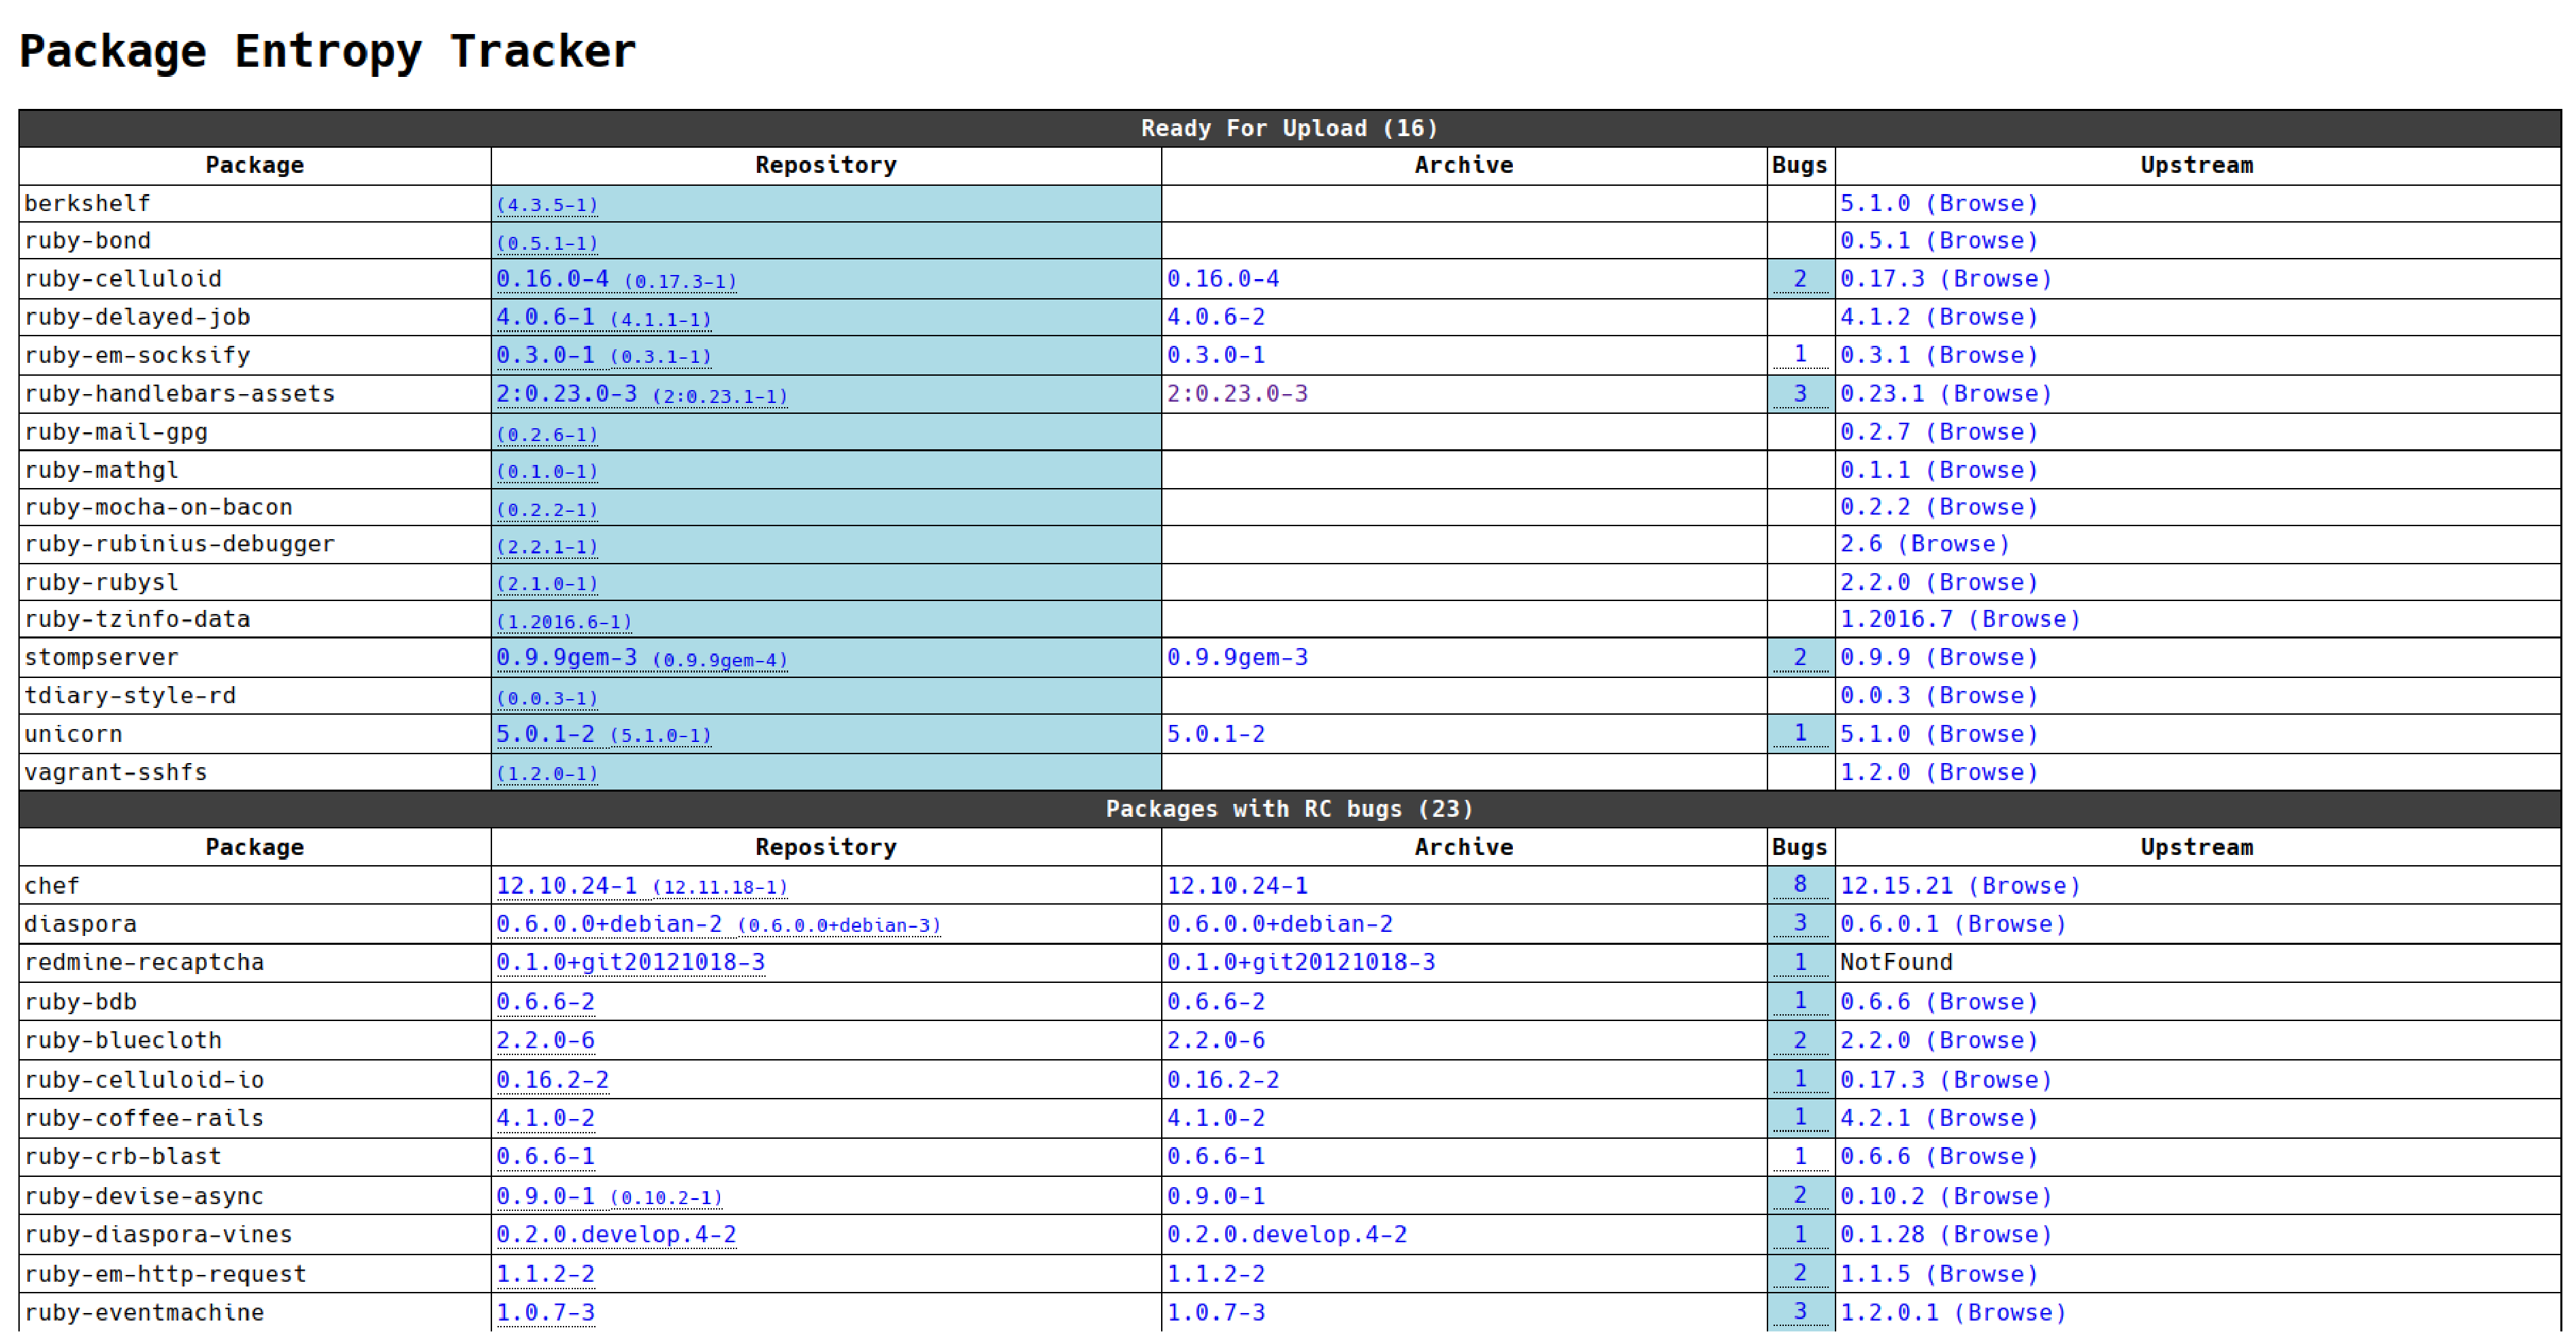
\includegraphics[scale=0.25]{figuras/pet1.eps}
	\caption{Visão geral do Pet utilizado pelo time de ruby}
\end{figure}

O \textit{Pet} é uma aplicação escrita em python, e que hoje é mantida pela Universidade de Brasília. O Pet faz uso de uma técnica chamada de ORM(\textit{Object Relational Mapping}). 
Nesse tipo de técnica, orientada a objetos, uma classe da camada modelo é mapeada diretamente por uma tabela em um banco de dados relacional, criando um nível de abstração entre o banco de dados, e a modelagem de negócio da aplicação.
Isso permite que a aplicação faça buscas complexas no banco de dados a partir de uma DSL(\textit{Domain Specific Language}), sem a necessidade da escrita direta de código sql dentro da aplicação.

Hoje, o banco de dados do Pet está organizado da seguinte forma:
\begin{figure}[h]
	\centering
	\label{fig01}
        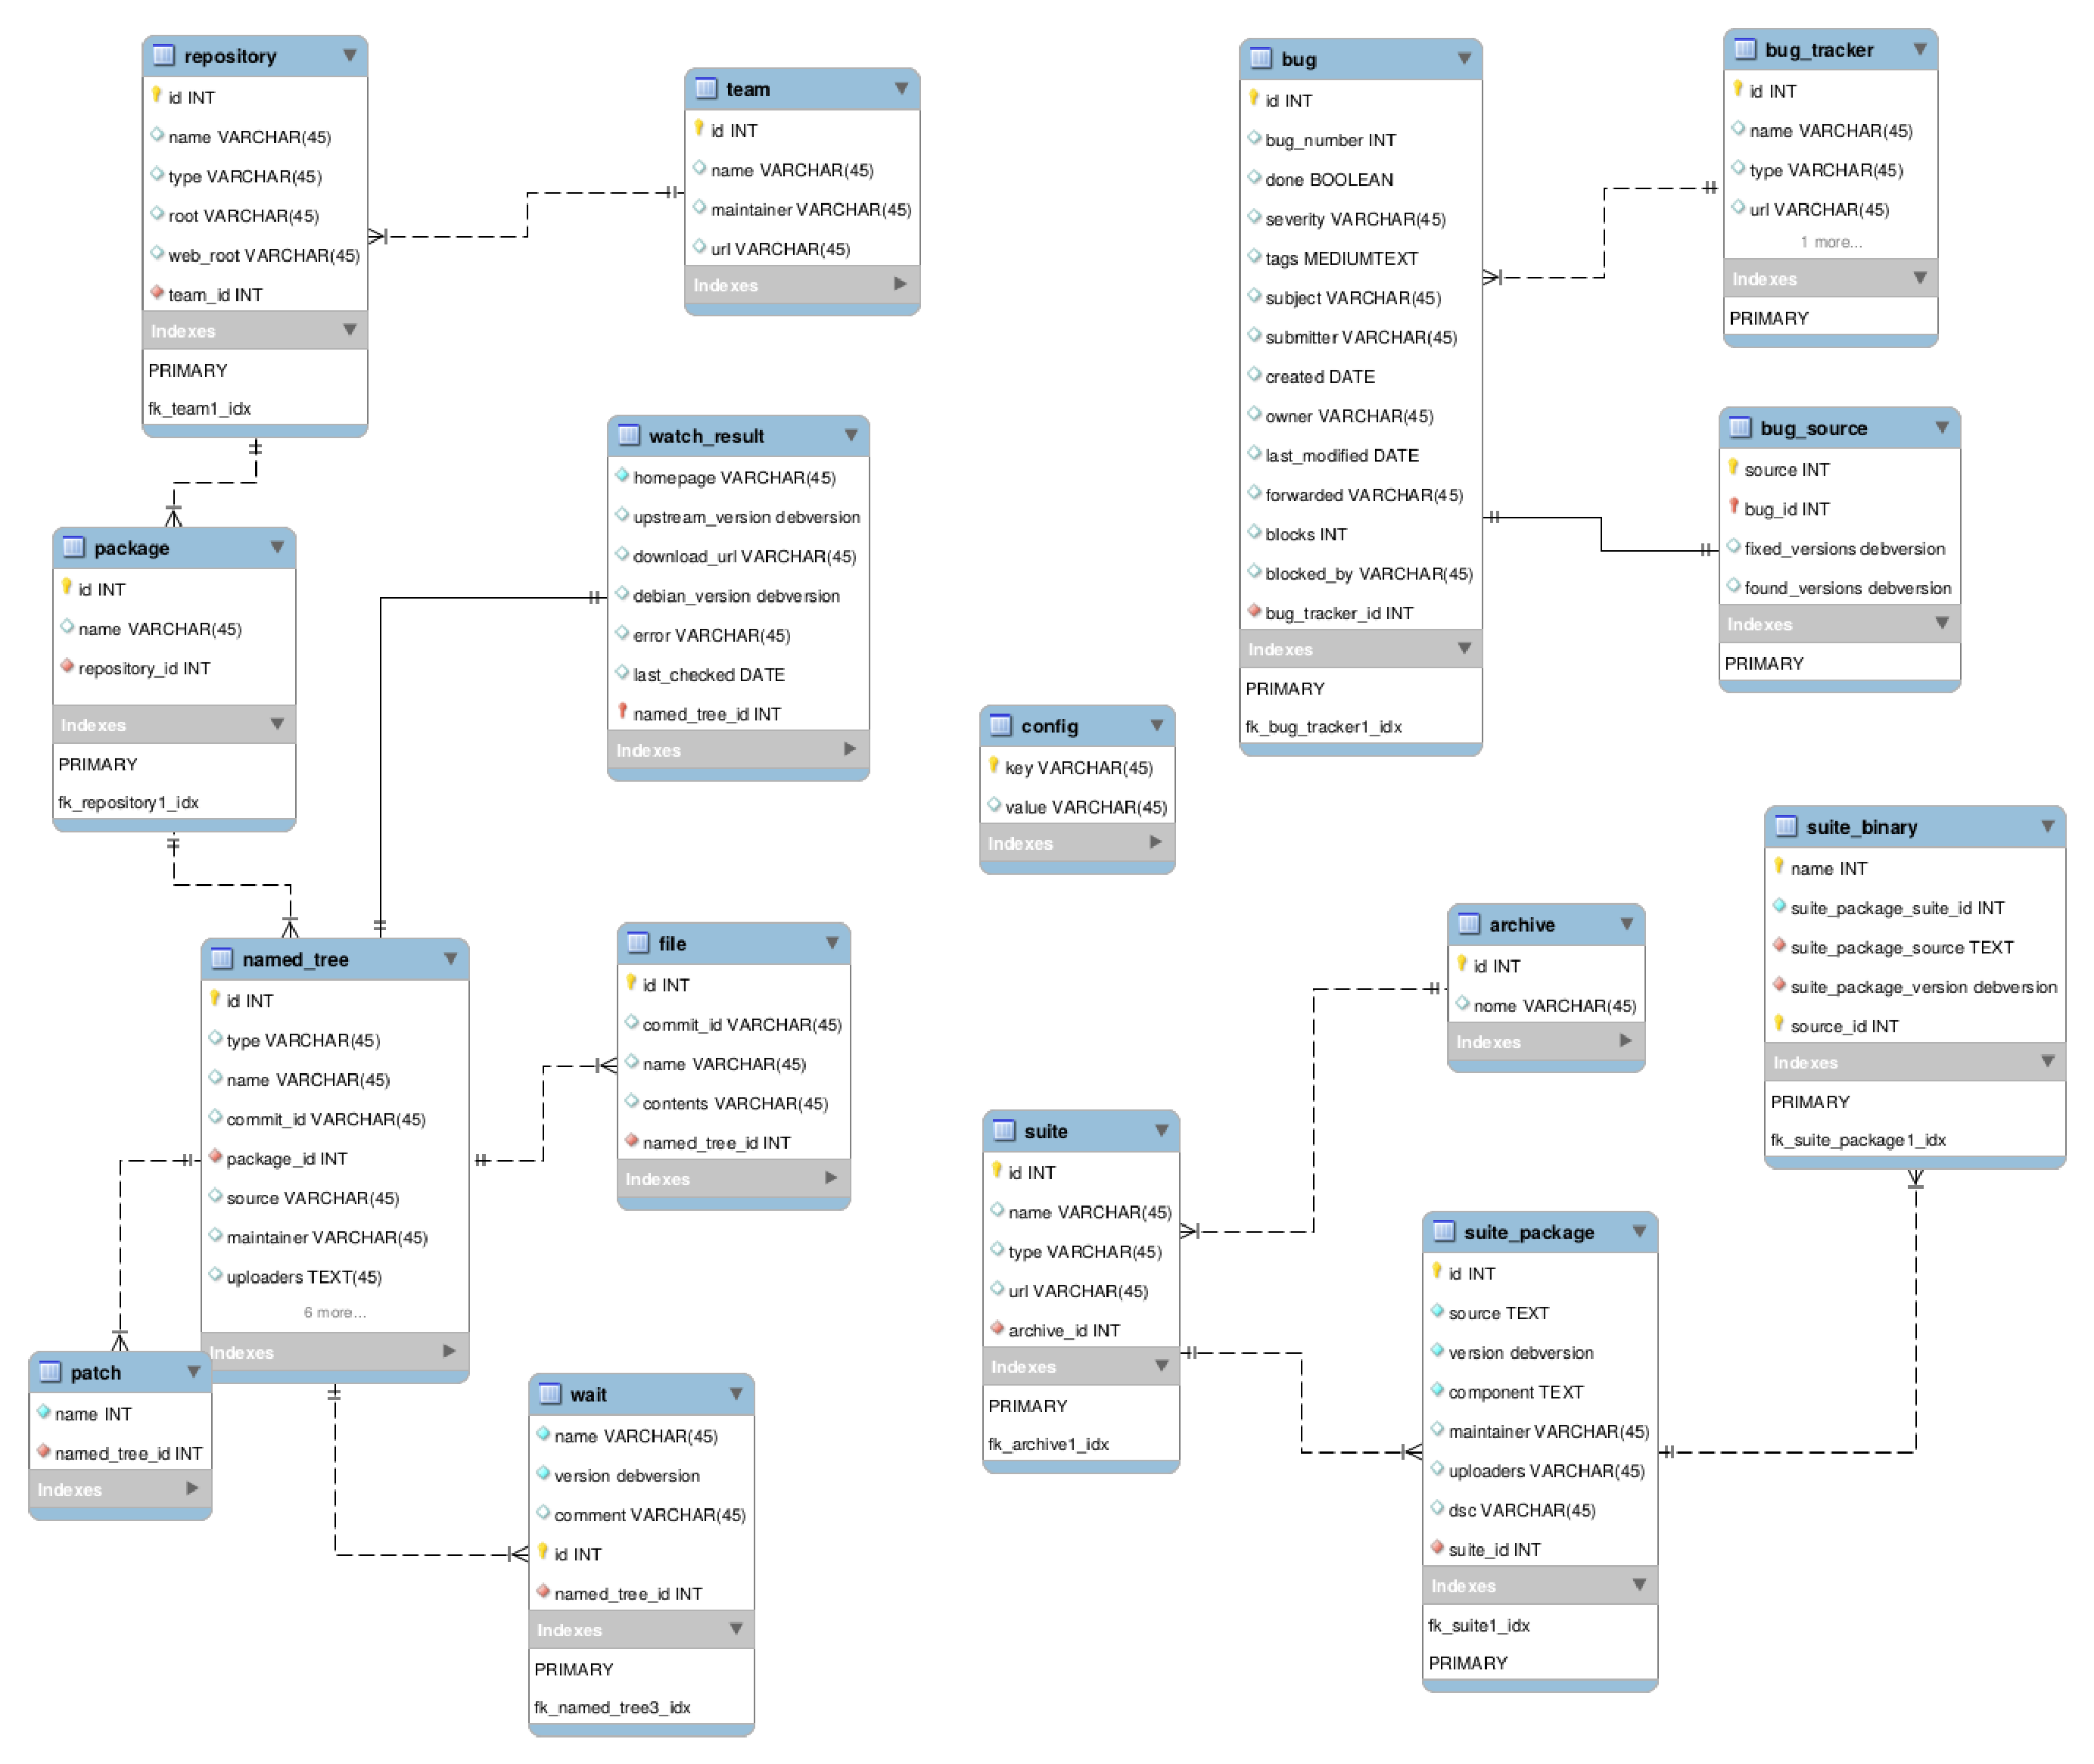
\includegraphics[scale=0.33]{figuras/base1.eps}
	\caption{Base de dados do Pet}
\end{figure}


\subsection{Debci}

\subsection{Lintian}

\section{Modelo de dados}

\section{Análise Estatística}

\section{Limitações do trabalho}
